\subsubsection{SPS-Programmierung}
In der Automatisierungstechnik werden speicherprogrammierbare Steuerungen (SPS) zur Realisierung unterschiedlichster Abläufe eingesetzt.  
Um die gewünschten Funktionen zur Automatisierung von Prozessen umzusetzen, ist es erforderlich, diese Abläufe in Form eines Programms in die Steuerung zu implementieren.

Ein SPS-Programm folgt dabei in der Regel einem klar strukturierten Aufbau \cite{Seitz.2021}:
\begin{itemize}
	\item Definition der Ein-, Ausgangs- und Hilfsvariablen in einer Variablentabelle,
	\item Programmierung des Hauptprogramms mit den zugehörigen Unterprogrammen und Funktionsbausteinen,
	\item Kompilierung des Programms und Übertragung in die Steuerung.
\end{itemize}

\begin{figure}[H]
	\centering
	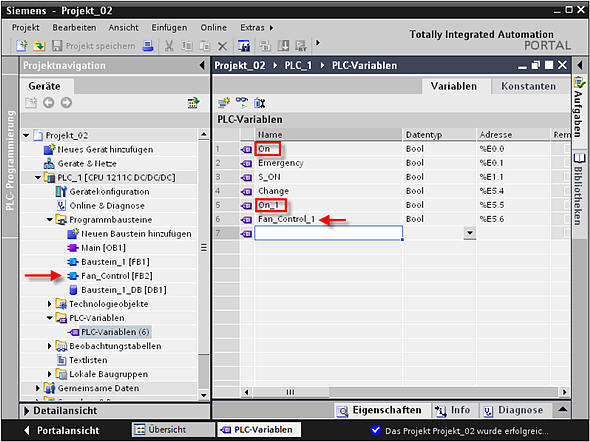
\includegraphics[width=0.8\linewidth]{images/Variablentabelle.jpg}
	\caption{Übersicht der Variablentabelle in TIA Portal \cite{siemens_vars2024}}
	\label{fig:uebersicht_tia}
\end{figure}

Das Hauptprogramm besteht aus sogenannten \textbf{POUs} (Program Organization Units, deutsch: Programmorganisationseinheiten).  
Diese werden in drei Arten unterteilt: \textbf{Programme}, \textbf{Funktionen (FC)} und \textbf{Funktionsbausteine (FB)}.  
Die Realisierung dieser POUs in \textit{Siemens TIA Portal} wurde bereits im vorherigen Kapitel (vgl. \ref{label}) beschrieben.  
Nachfolgend wird die Bedeutung und Funktion der einzelnen Organisationseinheiten erläutert.

Das \textbf{Programm} dient der Realisierung komplexer Abläufe, beispielsweise von Schrittketten oder Hauptlogiken.  
Eine \textbf{Funktion (FC)} ist mit einer C-ähnlichen Funktion vergleichbar. Sie verarbeitet eine oder mehrere Eingangsvariablen und gibt nach der Abarbeitung ein Ergebnis zurück.  
Gemäß IEC 61131-3 können Funktionen jedoch nicht rekursiv aufgerufen werden und besitzen kein eigenes Speicherverhalten, d.\,h. sie können keine Werte dauerhaft speichern \cite{Seitz.2021}.  
Ein einfaches Beispiel hierfür ist ein logisches \textbf{UND-Gatter}.

Ein \textbf{Funktionsbaustein (FB)} hingegen besitzt ein internes Gedächtnis und kann Werte über mehrere Zyklen hinweg speichern. Dadurch eignet er sich besonders für Zustandsautomaten oder speichernde Operationen.  
Ein klassisches Beispiel hierfür ist ein \textbf{RS-Flip-Flop}.

Für die Programmierung stehen verschiedene Sprachen nach IEC 61131-3 \cite{IEC6113-3_2022} zur Verfügung:
\begin{itemize}
	\item KOP (Kontaktplan),
	\item AWL (Anweisungsliste),
	\item FUP/FBS (Funktionsplan / Funktionsbausteinsprache),
	\item ST/SCL (Structured Text / Structured Control Language)\footnote{SCL ist die Siemens-spezifische Implementierung der nach IEC~61131-3 genormten Programmiersprache Structured Text (ST) im TIA Portal \cite{Kanngießer}.}
\end{itemize}

In modernen Industrieanlagen werden überwiegend \textbf{FUP} und \textbf{ST} eingesetzt. Diese Programmiersprachen zeichnen sich durch eine gute Übersichtlichkeit und eine effiziente Fehleranalyse aus.  
Trotzdem bestehen zwischen beiden Varianten wesentliche Unterschiede, die in Tabelle~\ref{tab:vergleich_fup_st} dargestellt sind.

\begin{table}[H]
	\centering
	\begin{tabular}{|p{7cm}|p{7cm}|}
		\hline
		\textbf{ST / SCL (Structured Text / Structured Control Language)} & \textbf{FUP (Funktionsplan)}\\
		\hline
		Textbasierte Programmiersprache & Grafische Programmiersprache\\
		\hline
		Hochsprachenähnlich (z.\,B. C, Pascal) & Verwendung grafischer Symbole und logischer Verknüpfungen\\
		\hline
		Klare und kompakte Struktur & Gefahr der Unübersichtlichkeit bei komplexen Programmen\\
		\hline
		Besonders geeignet für mathematische und logische Operationen & Gut geeignet für einfache logische Abläufe\\
		\hline
	\end{tabular}
	\caption{Vergleich zwischen ST (Structured Text) und FUP (Funktionsplan) \cite{siemens_programmieren}}
	\label{tab:vergleich_fup_st}
\end{table}

Wie aus der Tabelle hervorgeht, bietet die textbasierte Programmiersprache \textbf{ST} insbesondere bei komplexen Strukturen und mathematischen Berechnungen erhebliche Vorteile.  
\textbf{FUP} hingegen ist für Einsteiger leichter verständlich und eignet sich für überschaubare Steuerungslogiken.  
Mit zunehmender Komplexität der Abläufe stößt FUP jedoch schnell an seine Grenzen, da die grafische Darstellung umfangreicher Strukturen unübersichtlich werden kann \cite{siemens_programmieren}.  
Um die genauen Unterschiede zu erläutern, sollen zunächst grundlegende Elemente der einzelnen Sprachen eingeführt werden.  
Zunächst erfolgt eine Beschreibung der wichtigsten Grundbausteine in FUP.

\subsubsection*{Wichtige Grundfunktionen (UND, ODER, NICHT) in FUP}
\begin{figure}[H]
	\centering
	\begin{subfigure}[b]{0.49\textwidth}
		\centering
		\includegraphics[width=0.8\linewidth]{images/UND_GATTER}
		\caption{\textbf{UND\_Gatter} \cite{Hering}}
	\end{subfigure}
	\hfill
	\begin{subfigure}[b]{0.49\textwidth}
		\centering
		\includegraphics[width=0.8\linewidth]{images/ODER_GATTER}
		\caption{\textbf{ODER\_Gatter} \cite{Hering}}
	\end{subfigure}
	
	\vspace{1cm}
	
	\begin{subfigure}[b]{0.49\textwidth}
		\centering
		\includegraphics[width=0.8\linewidth]{images/NOT_GATTER}
		\caption{\textbf{NOT\_Gatter} \cite{Hering}}
	\end{subfigure}
	\caption{Darstellung der logischen Grundfunktionen in FUP}
	\label{fig:grundfunktionen_fup}
\end{figure}

\subsubsection*{Wichtige Funktionsbausteine in FUP}
\begin{figure}[H]
	\centering
	\begin{subfigure}[b]{0.49\textwidth}
		\centering
		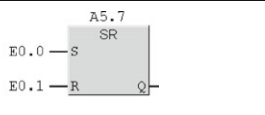
\includegraphics[width=0.8\linewidth]{images/SR_FLIPFLOP}
		\caption{\textbf{SR\_FLIPFLOP} \cite{Hering}}
	\end{subfigure}
	\hfill
	\begin{subfigure}[b]{0.49\textwidth}
		\centering
		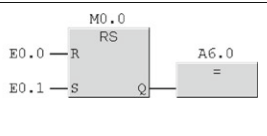
\includegraphics[width=0.8\linewidth]{images/RS_FLIPFLOP}
		\caption{\textbf{RS\_FLIPFLOP} \cite{Hering}}
	\end{subfigure}
	
	\vspace{1cm}
	
	\begin{subfigure}[b]{0.49\textwidth}
		\centering
		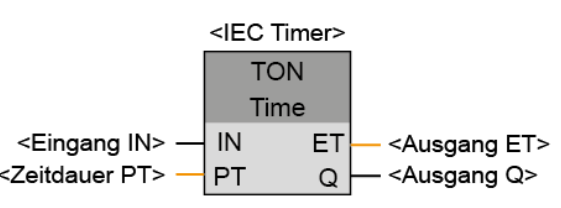
\includegraphics[width=0.8\linewidth]{images/TON}
		\caption{\textbf{Einschaltverzögerung (TON)} \cite{Hering}}
	\end{subfigure}
	\hfill
	\begin{subfigure}[b]{0.49\textwidth}
		\centering
		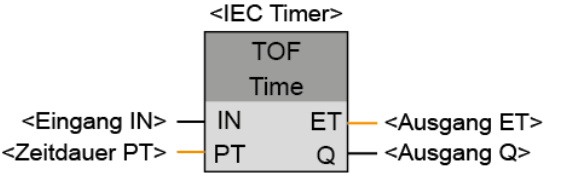
\includegraphics[width=0.8\linewidth]{images/TOF}
		\caption{\textbf{Ausschaltverzögerung (TOF)} \cite{Hering}}
	\end{subfigure}
	\caption{Darstellung wichtiger Funktionsbausteine in FUP}
	\label{fig:funktionsbausteine_fup}
\end{figure}

In den obigen Abbildungen sind die wichtigsten Grundfunktionen und Funktionsbausteine in \textbf{FUP} dargestellt.  
Mit diesen können diverse Abläufe realisiert werden, wie beispielsweise einfache Förderbandsteuerungen.  
Komplexe, lange Abläufe sind jedoch sehr aufwendig zu realisieren. Für eine SPS ist es daher gebräuchlich, hierfür auf \textbf{ST/SCL} auszuweichen.  
In FUP können ebenfalls mathematische Operationen durchgeführt werden. Für Berechnungen existieren spezielle Bausteine. Allerdings ist es schwierig, längere Rechenvorgänge übersichtlich darzustellen, da die Struktur schnell unübersichtlich wird.  
Aus diesem Grund werden für sämtliche mathematische Operationen häufig Berechnungen in \textbf{ST/SCL} durchgeführt.  
Beim vorliegenden Modell, dem Hochregallager, wurde beispielsweise die Positionsermittlung der Lagerplätze für das automatisierte Einlagern im vergangenen Studienprojekt in \textbf{SCL} realisiert.
\subsubsection*{Grundlegende Anweisungen in SCL}
Im vorliegenden Projekt wird mit einer Siemens SPS gearbeitet. Somit ist SCL (Structured Control Language) der Standard im Bereich textbasierte Programmierung.\\
Hierbei gibt es einige konkrete Anweisungen, welche eine übersichtliche Programmierung gewährleisten.\\
Zu diesen zählen:
\begin{itemize}
	\item \textbf{Zuweisungen:} \texttt{Variable := Wert;}  
	Beispiel: \texttt{Motor\_Start := TRUE;}
	\item \textbf{Bedingte Anweisungen (IF-Strukturen):}  
	\texttt{IF Sensor = TRUE THEN Motor := TRUE; END\_IF;}
	\item \textbf{Mehrzweigige Bedingungen (IF-ELSIF-ELSE):}  
	\texttt{IF Temp > 50 THEN Alarm := TRUE; ELSIF Temp > 30 THEN Warning := TRUE; ELSE Alarm := FALSE; END\_IF;}
	\item \textbf{Schleifenstrukturen:}  
	\texttt{FOR i := 1 TO 5 DO Count := Count + 1; END\_FOR;}
	\item \textbf{Vergleiche und logische Operatoren:}  
	\texttt{AND, OR, NOT, >, <, =, >=, <=}
\end{itemize}